%=====================================================================
\section{Introduction}
%=====================================================================
Predator--prey interactions are the textbook example of a nonlinear dynamic system. The Lotka--Volterra
(LV) equations \cite{lotka1925,volterra1926} predict neutral cycles around an equilibrium whose prey level is
set by predator parameters and vice versa. Their structural fragility is equally classic: adding prey
self-limitation turns the centre into a stable focus, a saturating (type~II) functional response can
destabilise it into a limit cycle \cite{rosenzweig1963}, and enrichment of the prey's resource pushes the
system across that boundary, the \emph{paradox of enrichment} \cite{rosenzweig1971}. Real and simulated
populations add two ingredients the ODEs ignore: demographic noise, which can sustain oscillations in an
otherwise damped system \cite{mckane2005}, and space, which lets local extinctions be recolonised and was
shown experimentally to permit persistence \cite{huffaker1958}. Lattice predator--prey models have long been
used to study these effects \cite{durrett1994,pascual1999}, and individual-based teaching models such as the
NetLogo wolf--sheep model \cite{wilensky1997} are widely used in classrooms.

This paper uses a deliberately simple lattice ABM for a different purpose: to make the vocabulary of
systems and control---state, feedback loop, equilibrium, stability, delay, nonlinearity, model reduction,
open- versus closed-loop control, and objective design for optimisation---\emph{measurable} in a single
system that students can run in a browser. We ask three questions.
\begin{enumerate}[nosep,leftmargin=*]
  \item \textbf{Dynamics.} Which qualitative regimes do the rules produce, and how do they depend on the
        predator starvation time $N$, the resource regrowth time $R$ and system size?
  \item \textbf{Reduction.} When does a two- or three-variable LV model, with rates estimated from the
        ABM's own event counts, describe the agent dynamics, and what does it miss?
  \item \textbf{Control.} With harvesting as the input, how do open-loop (constant quota, constant
        effort) and closed-loop (proportional feedback) policies trade yield against stability?
\end{enumerate}
We complement parameter sweeps with an evolutionary quality-diversity search over 18 parameters, which
also illustrates a lesson every control engineer learns: optimisers exploit the objective you wrote, not
the one you meant.

%=====================================================================
\section{Model}
%=====================================================================
The world is an $L\times L$ torus ($L=200$ unless stated). Each cell has a \emph{vegetation layer}
(grown or regrowing; a fraction of cells may be barren) and an \emph{animal layer} holding at most one
animal: empty, prey or predator. Animals carry a hunger counter and an age. One tick executes, in order:
\begin{enumerate}[nosep,leftmargin=*]
  \item \textbf{Regrowth.} A grazed fertile cell regrows exactly $R$ ticks later.
  \item \textbf{Movement.} Prey, then predators, move to a free Moore neighbour. With probability $0.7$ the
        move is directed: prey maximise local vegetation minus $5\times$ local predator density
        (sensing radius 3); predators maximise local prey density (radius 4). Otherwise the move is random.
  \item \textbf{Predation.} Each predator kills prey in its Moore neighbourhood, at most one per tick
        (satiation).
  \item \textbf{Grazing.} Each prey eats up to $K$ grown cells in its $3\times3$ neighbourhood (own cell first);
        it is \emph{fed} if it ate $K$ ($K=1$ here).
  \item \textbf{Hunger and ageing.} Unfed prey increment hunger and die at $S$ ($=6$); predators without a kill
        increment hunger and die at $N$ ($=12$ by default). Optional maximum ages.
  \item \textbf{Reproduction.} A fed prey reproduces with probability $0.08$, a predator that killed with
        probability $0.3$, into a random free neighbour.
  \item \textbf{Harvest (control input).} $u$ animals of the harvested species are removed at random:
        constant effort $u=\mathrm{Bin}(n,E)$, constant quota $u=\min(Q,n)$, or proportional feedback
        $u=\mathrm{clip}\big(\lfloor K_p(n-r)\rceil,\,0,\,n\big)$ with set point $r$, switched on at a given tick.
\end{enumerate}
Initial densities are $60\%$ vegetation, $6\%$ prey and $1\%$ predators. Conflicts (two agents targeting one
cell) are resolved in random order; runs are reproducible from a seed. The model is vectorised in NumPy
($\approx\!3$\,ms per tick at $200^2$). We record per tick the counts $x$ (prey), $y$ (predators), $v$
(vegetation) and every event: births, kills, starvation, age deaths, cells grazed and regrown, and harvest.
The event identity $x_{t+1}=x_t+\text{births}-\text{kills}-\text{starved}-\text{aged}-\text{harvested}$ is
checked by the test suite.

%=====================================================================
\section{Methods}
%=====================================================================
\paragraph{Metrics.} Statistics use the second half of each run (after the transient): mean, coefficient
of variation (CV, oscillation amplitude), dominant period (first autocorrelation maximum after the first
zero crossing, accepted if $>0.1$), predator lag (argmax of the prey--predator cross-correlation), and
outcome (coexistence, predator extinction, total extinction). Periods are reported only for coexisting runs
with prey CV $\ge 0.05$. Unless stated, each condition uses 5--10 seeds and 3000 ticks.

\paragraph{LV family and event-based fitting.} With $x,y,v$ as densities per cell, we consider
classic LV ($\dot x=ax-bxy$, $\dot y=cbxy-gy$), logistic LV ($ax\to rx(1-x/K)$), Rosenzweig--MacArthur
(RM; $bxy\to axy/(1+ahx)$), and a three-level chain
$\dot v=\rho(V-v)-evx$, $\dot x=\varepsilon evx-\mu x-bxy$, $\dot y=cbxy-gy$.
Instead of fitting trajectories, which drift out of phase for noisy cycles, each rate is a regression of the
matching event count on the pre-tick state, e.g.\ kills $\approx b\,x\,y$, predator births $\approx c\cdot$kills,
predator deaths $\approx g\,y$ (RM via Gauss--Newton). Unit tests recover known rates exactly from synthetic
histories. Models are integrated (RK4) from the ABM's initial state, and equilibria are classified by the
eigenvalues of the numerical Jacobian, giving a predicted period $2\pi/\mathrm{Im}\,\lambda$ and damping time
$-1/\mathrm{Re}\,\lambda$. We also derive, without fitting, a \emph{mean-field map} that applies the exact
rules to a well-mixed population (binomial neighbourhoods, hunger-class structure, delayed regrowth).

\paragraph{Experiments.} E1: seven regimes (Table~\ref{tab:regimes}). E2: $N\in[2,60]$, 17 values $\times$ 6
seeds. E3: $R\in[4,60]$ for $N=12$ and $30$. E4: $L\in[40,280]$ in two regimes, 10 seeds. E5:
quality-diversity search. E6: harvesting (effort, quota, feedback, open vs closed loop). E7: full model
comparison in two regimes. E8: shocks ($-50\%$ predators) at $t=1500$, 16 seeds per condition.

\paragraph{Optimisation.} A genome is a vector of 18 parameters in the unit hypercube (vegetation, prey and
predator traits, initial densities). Each genome is simulated on 3 training seeds (common random numbers),
$100^2$ cells, 1500 ticks. Fitness for \emph{robust coexistence} is mean survival fraction
$+\,0.5\times$resilience (minimum/mean population after the transient) $-0.25\times$ the std of survival.
MAP-Elites \cite{mouret2015} keeps the fittest genome in each cell of a $12\times12$ behaviour grid
(prey CV $\times$ prey period); offspring arise by BLX-$\alpha$ crossover and Gaussian mutation of archive
members. The top genomes are re-validated on 10 hold-out seeds. A target-free objective is also offered for
harvest yield (Sec.~\ref{sec:yield}).

%=====================================================================
\section{Results}
%=====================================================================
\subsection{Regimes}
The rules produce a rich set of behaviours (Fig.~\ref{fig:regimes}, Table~\ref{tab:regimes}). With default
parameters the populations settle to a noisy equilibrium of $\approx\StablePrey$ prey and $\StablePred$
predators (prey CV \StableCV). Raising $N$ from 12 to 30 produces sustained cycles (CV \CycleCV, period
$\approx\CyclePeriod$ ticks) in which predators lag prey by $\approx\CycleLag$ ticks, close to the quarter
period expected for LV dynamics. Spatially, the cycles appear as travelling fronts of prey invading
vegetation and predators following them (Fig.~\ref{fig:snapshots}). Cutting the predation loop ($N=3$)
leaves prey limited only by vegetation at $\approx\PreyOnlyK$; overly efficient predators eat all prey and
then starve.

\begin{figure*}[!tp]
\centering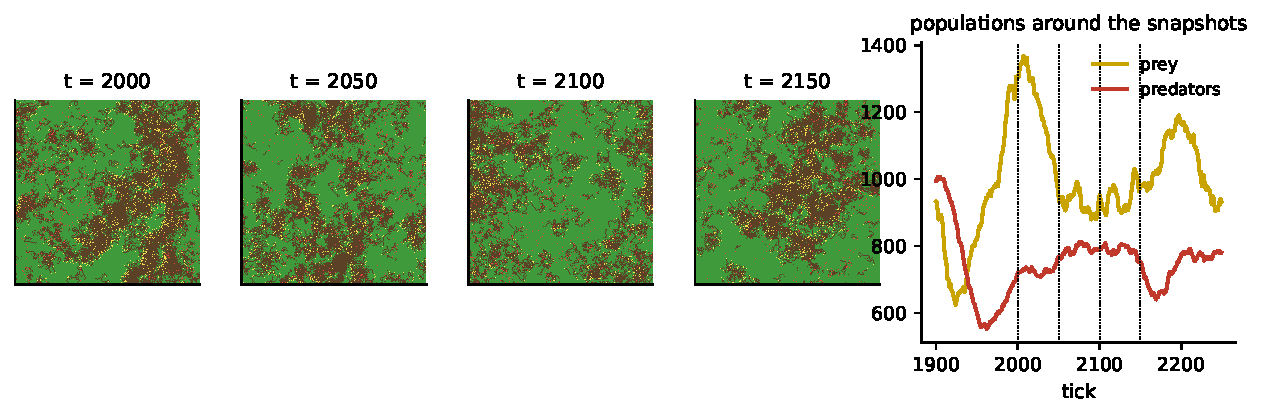
\includegraphics[width=\linewidth]{snapshots.pdf}
\caption{Cycling regime ($N=30$). Grid snapshots (green vegetation, brown regrowing soil, yellow prey, red
predators) during one cycle and the corresponding population curves.}
\label{fig:snapshots}
\end{figure*}

\begin{table*}[!tp]
\centering\small
\caption{Regimes (E1): $200^2$ cells, 3000 ticks, 6 seeds. Means and CV over the second half; period
only where prey CV$\ge0.1$ (visible oscillations). ``Prey only'' has no predators by design;
for total extinction the extinction tick is given.}
\label{tab:regimes}
\begin{tabular}{llrrrrr}
\toprule
Regime & Change from defaults & Typical outcome & Prey & Predators & Prey CV & Period \\
\midrule
\tabinput{table_regimes.tex}
\bottomrule
\end{tabular}
\end{table*}

\begin{figure}[!htbp]
\centering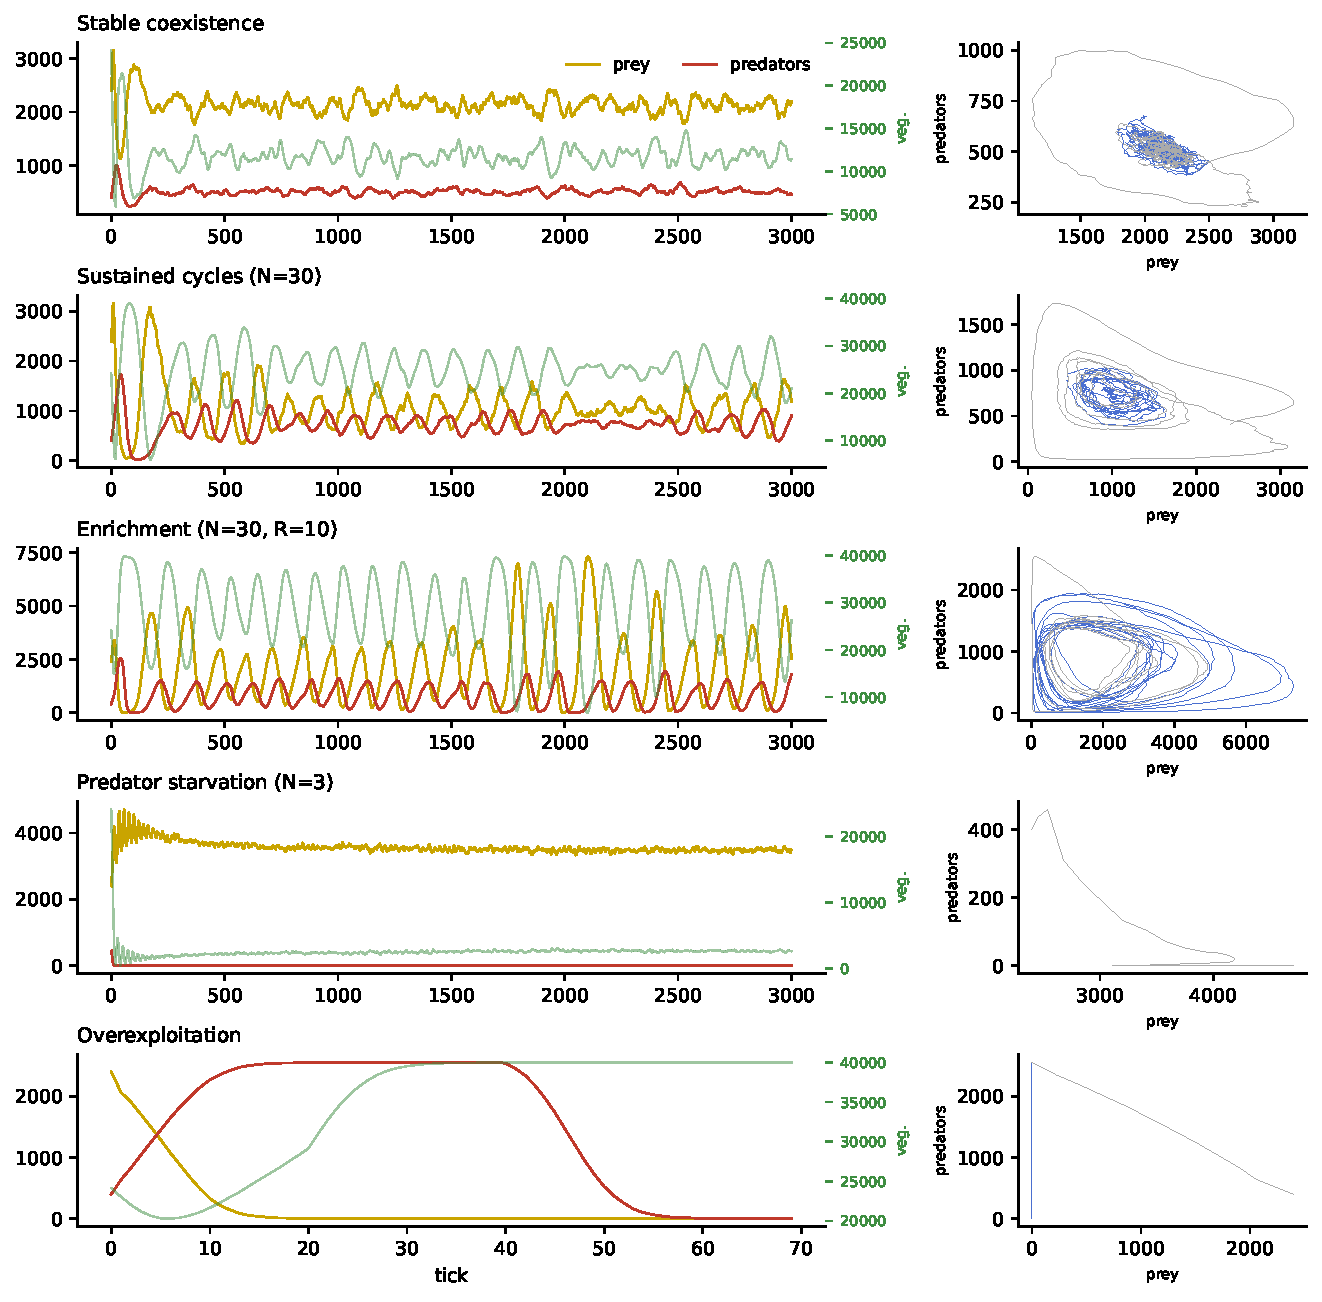
\includegraphics[width=\linewidth]{regimes.pdf}
\caption{Time series (left; vegetation on the right axis) and phase portraits (right; grey early, blue late)
for five regimes.}
\label{fig:regimes}
\end{figure}

\subsection{Predator starvation time sets the regime}
Figure~\ref{fig:starve} sweeps $N$. Coexistence is certain for $\NcoexMin\le N\le\NcoexMax$. For
$N\le\NpredExt$ predators cannot bridge the time between kills and go extinct, after which prey sit at the
vegetation-limited carrying capacity. At $N=\NoverMin$ only \NoverPcoex\% of seeds coexist: long-lived
predators overshoot and collapse their food supply (overexploitation).

Inside the window, mean prey fall from \PreyNtwelve{} at $N=12$ to \PreyNforty{} at $N=40$ while predators
saturate at $\approx\PredPlateau$. This is the LV signature: the prey equilibrium $x^\ast=g/(cb)$ depends on the
predator death rate $g$, which falls with $N$, whereas $y^\ast$ is set by prey production. The equilibria of
the fitted chain model reproduce the ABM means with a mean error of \EqErrMean\% (maximum \EqErrMax\%;
Fig.~\ref{fig:starve}b).

\begin{figure*}[!tp]
\centering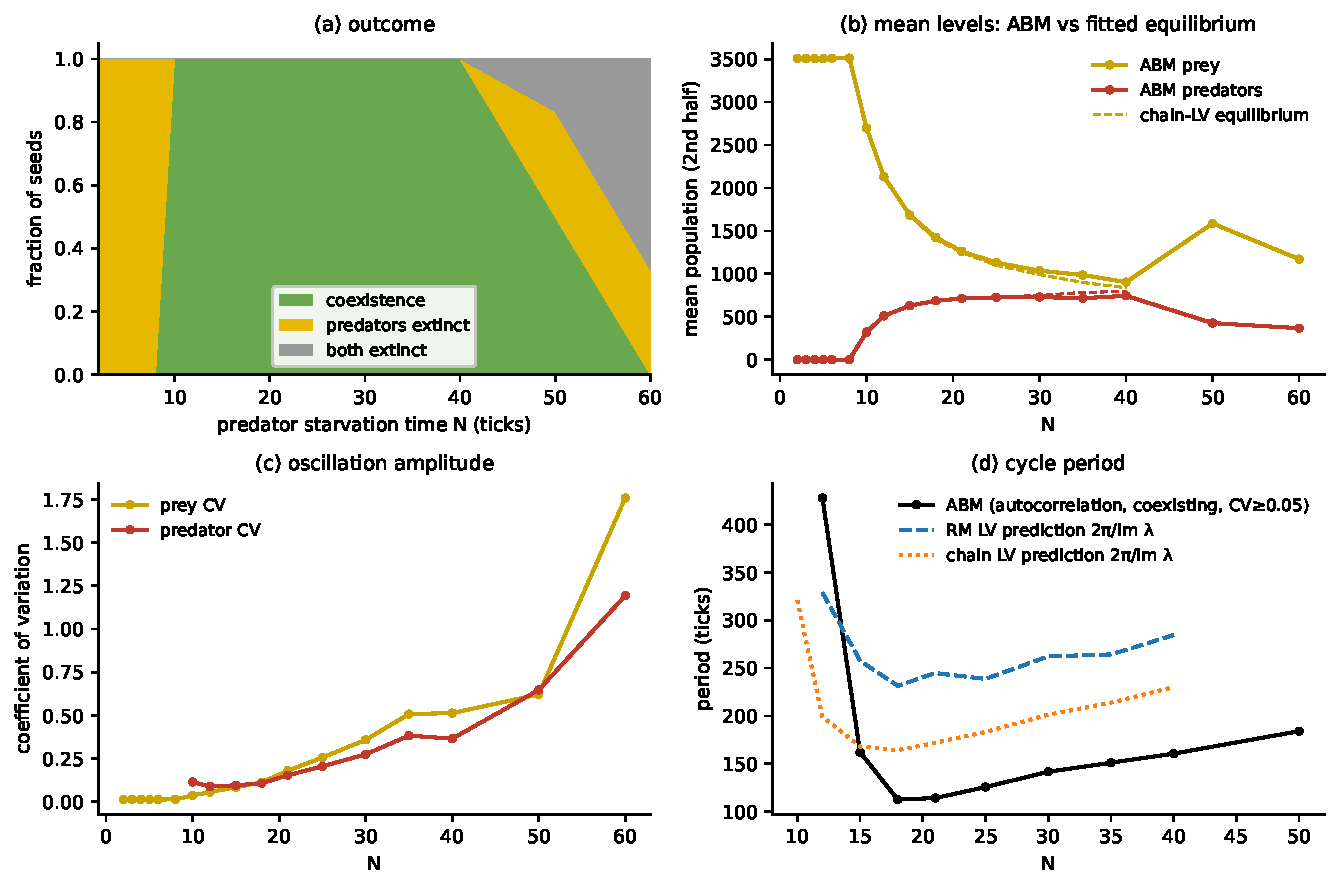
\includegraphics[width=0.85\linewidth]{starve_sweep.pdf}
\caption{Sweep of predator starvation time $N$ (E2; 6 seeds per point, 3000 ticks, $200^2$).
(a) Outcomes. (b) Mean populations vs equilibria of the fitted chain model (dashed). (c) Oscillation
amplitude. (d) Cycle period of the ABM vs the eigenvalue predictions of the fitted RM and chain models.}
\label{fig:starve}
\end{figure*}

\subsection{Damped models, sustained cycles}\label{sec:quasi}
The oscillation amplitude grows smoothly with $N$, from a prey CV of \CVlow{} to \CVhigh{}
(Fig.~\ref{fig:starve}c); there is no sharp onset. Every fitted logistic, RM and chain model in the window
has a \emph{stable focus}, i.e.\ predicts that oscillations decay. Table~\ref{tab:lv} and Fig.~\ref{fig:lv}
show the cycling regime in detail: all fitted models get the means right, the deterministic ones relax to
equilibrium, and classic LV oscillates only because it is neutrally stable, with an amplitude (CV
\CclassicCV) that depends on initial conditions rather than dynamics. The ABM's cycles are therefore best
understood as \emph{noise-sustained quasi-cycles} \cite{mckane2005}: demographic noise continually excites a
weakly damped mode. Increasing $N$ weakens predator mortality, which pushes the leading eigenvalue towards the
imaginary axis (fitted RM damping time \SrmTau{} ticks at $N=12$ vs \CrmTau{} at $N=30$), so the same noise
produces larger oscillations.

The ABM cycles are also faster: periods of \ABMperLo--\ABMperHi{} ticks for $N\ge15$ against
\ChainperLo--\ChainperHi{} (chain) and \RMperLo--\RMperHi{} (RM) predicted from the eigenvalues
(Fig.~\ref{fig:starve}d). ODEs replace the fixed starvation delay by an exponential death rate $g$; a
constant $g$ explains only $R^2=\CgRsq$ of the per-tick predator deaths. A delayed death process shortens
the feedback loop's response compared with the exponential approximation of the same mean lifetime.

\begin{table}[!htbp]
\centering\small\setlength{\tabcolsep}{3.5pt}
\caption{Cycling regime ($N=30$, seed 42, 3000 ticks): ABM vs models fitted to its events. Stability from
the Jacobian at equilibrium; period from the eigenvalues where available.}
\label{tab:lv}
\begin{tabular}{lcrrrr}
\toprule
 & Equil. & Prey & Pred. & CV & Period\\
\midrule
\tabinput{table_lv.tex}
\bottomrule
\end{tabular}
\end{table}

\begin{figure}[!htbp]
\centering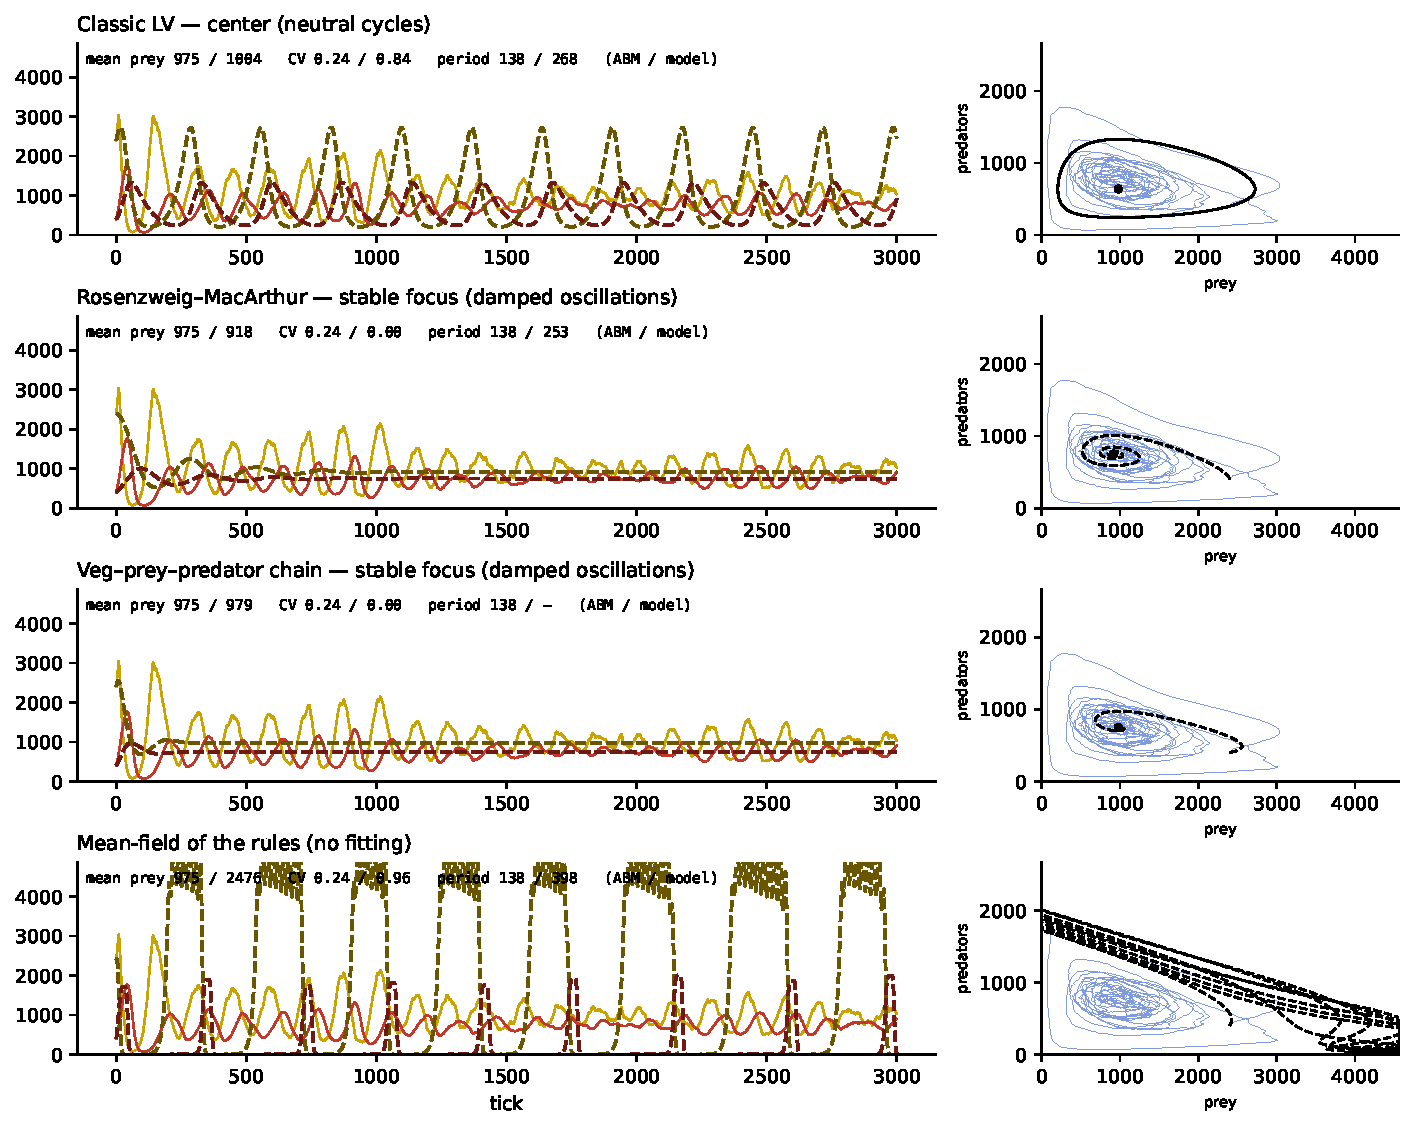
\includegraphics[width=\linewidth]{lv_compare.pdf}
\caption{ABM (solid) vs models (dashed) in the cycling regime, with phase portraits. Numbers: ABM / model.}
\label{fig:lv}
\end{figure}

\subsection{Space is stabilising}
In a well-mixed population a predator with eight neighbour cells meets prey at rate $\approx 8x$, so
$b\approx8$. The rate fitted from kills in the ABM is \bLo--\bHi{} across the coexistence window, a
\bRatio-fold reduction (Fig.~\ref{fig:spatial}): predators deplete their surroundings and must move to
find new prey, while prey that escape form clusters behind the front. The mean-field map of the same rules,
which assumes mixing, is wildly oscillatory (prey CV $\ge\MFcvLo$ in the whole window, against \CVlow--\CVhigh{} in
the ABM) and keeps predators near extinction between outbreaks (mean \SmfPred{} vs \StablePred{} in the
stable regime). Local depletion thus acts as a distributed negative feedback that the well-mixed
description lacks \cite{pascual1999}.

\begin{figure}[!htbp]
\centering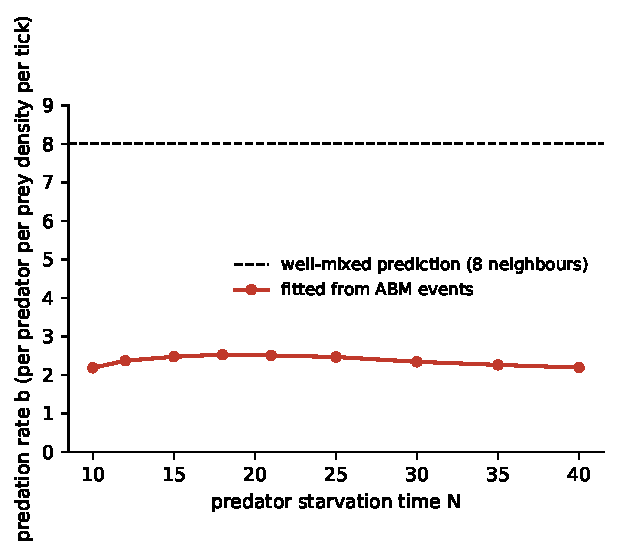
\includegraphics[width=0.9\linewidth]{spatial_rate.pdf}
\caption{Predation rate $b$ fitted from ABM kill events vs the well-mixed prediction.}
\label{fig:spatial}
\end{figure}

\subsection{Enrichment: coexistence is bounded on both sides}
Shortening the regrowth time $R$ enriches the prey's resource (Fig.~\ref{fig:enrich}). For $N=12$ the prey
CV rises from \EnrAcvPoor{} at $R=\EnrRpoor$ (where predators are already extinct) to \EnrAcvRich{} at
$R=\EnrRrich$, and peak prey reach $\approx\EnrAmaxRich$. In the cycling regime ($N=30$) the effect is
stronger and lethal: amplitude grows to CV $\approx\EnrBcvRich$, and coexistence drops to as low as
\EnrBpMin\% of seeds at $R=\EnrBRworst$ (boom--bust cycles drive predators, and sometimes prey, to
extinction). This is the paradox of enrichment \cite{rosenzweig1971} reproduced by agents, with a
qualitative difference from the RM model: here destabilisation is gradual and acts by amplifying
stochastic troughs until one hits zero, rather than through a sharp Hopf bifurcation. On the poor side,
slow regrowth ($R\ge28$ for $N=12$, $R=60$ for $N=30$) keeps prey too sparse to sustain predators
(bottom-up control). Coexistence thus occupies an intermediate band of resource productivity whose width
shrinks as predators become more persistent. Richer resources also raise the mean prey level, which a
chain model with a fixed $x^\ast=g/(cb)$ cannot express; the shift reflects nonlinear averaging over
larger cycles.

\begin{figure*}[!tp]
\centering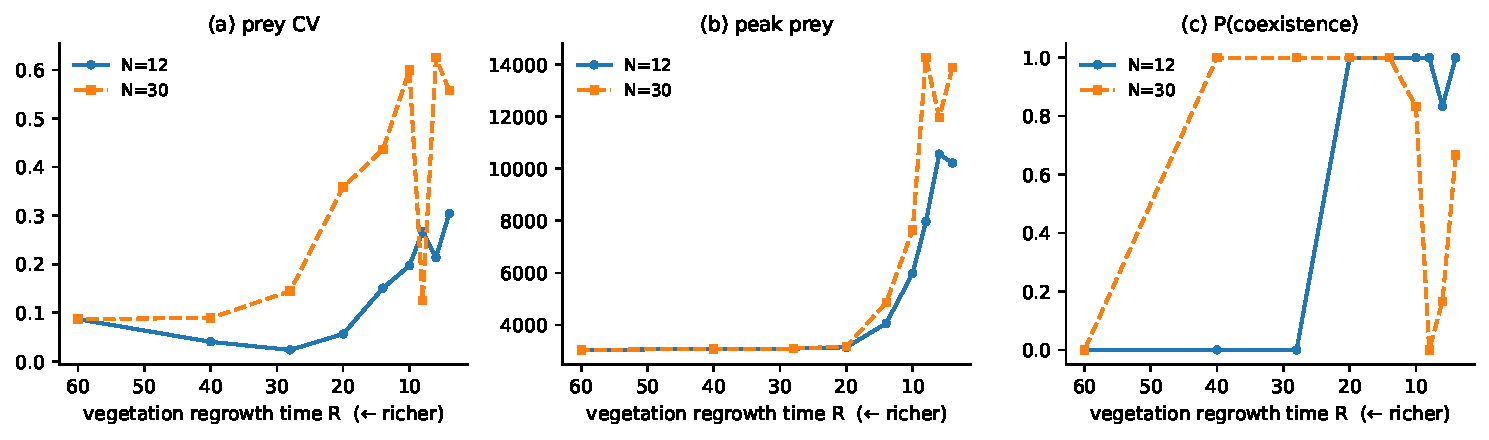
\includegraphics[width=0.9\linewidth]{enrichment.pdf}
\caption{Enrichment (E3; 6 seeds per point): vegetation regrowth time $R$ (richer to the right) for a
stable ($N=12$) and a cycling ($N=30$) predator.}
\label{fig:enrich}
\end{figure*}

\subsection{System size and demographic noise}
In the stable regime the prey CV scales as $(\text{cells})^{\SizeSslope}$ (Fig.~\ref{fig:size}a), the
$-\tfrac12$ law of independent demographic fluctuations: the deterministic equilibrium is approached as
the system grows, and the noisy wobble is a finite-size effect. The cycling regime decays more slowly
(exponent \SizeCslope{} over the sizes where it persists): its amplitude is set by the resonant
amplification of noise near a weakly damped mode as well as by system size. Persistence depends strongly
on size (Fig.~\ref{fig:size}b): the stable regime survives in \SizeSpSmall\% of $\SizeSLmin^2$ worlds and
in all worlds from $\SizeSLsafe^2$ cells, whereas the cycling regime never survives at $\SizeCLmin^2$ and
needs $\SizeCLsafe^2$ cells for certain persistence. Large oscillations combined with small populations
make extinction by a random trough likely, a stochastic analogue of an unstable equilibrium. (The
optimisation of Sec.~\ref{sec:opt} used $100^2$ cells, where even the cycling preset persists in only $80\%$ of runs;
its fitness therefore rewards robustness to this finite-size risk.)

\begin{figure}[!htbp]
\centering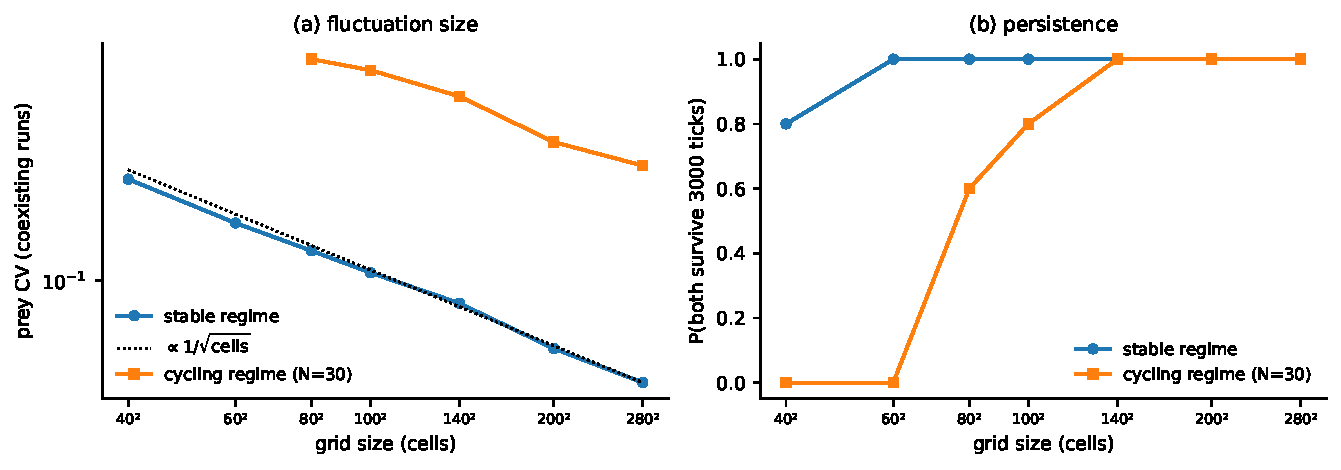
\includegraphics[width=\linewidth]{size.pdf}
\caption{System size (E4; 10 seeds). (a) Prey CV in coexisting runs; dotted: $\propto 1/\sqrt{\text{cells}}$.
(b) Probability that both species survive 3000 ticks.}
\label{fig:size}
\end{figure}

\subsection{Optimisation: the space of behaviours}\label{sec:opt}
The MAP-Elites search (\QDgens{} generations, population \QDpop, \QDevals{} simulations, with finite
lifespans of 150/300 ticks) filled \QDcells{} of \QDtotal{} behaviour cells (Fig.~\ref{fig:qd}). Coexistence
is possible from almost static populations to violent cycles in which prey vary many-fold
(CV up to $\approx1.4$; e.g.\ cell (10,6): CV \OscCV, period \OscPer, prey from \OscMin{} to \OscMax).
Fitness falls monotonically with amplitude, from \QDfitLowCV{} for CV$<0.125$ to \QDfitHighCV{} for
CV$\ge1.25$: a \emph{robustness--amplitude trade-off}, since deep troughs leave little margin before
extinction. The validated best genome (fitness \QDbest{} on 10 hold-out seeds) is a dense, nearly static
community (\QDbestPrey{} prey, \QDbestPred{} predators, CV \QDbestCV) with satiation raised to
\QDbestKills{} kills per tick.

\paragraph{Specification gaming.} A first search without lifespans and without a reproduction requirement
converged on a degenerate optimum: predators with zero reproduction probability and long starvation time,
i.e.\ a few dozen immortal predators living among prey that filled $94\%$ of the grid. It ``coexisted''
perfectly and contained no predator--prey dynamics at all, a textbook case of an optimiser exploiting an
incomplete objective \cite{lehman2020}. We excluded it by (i) imposing finite lifespans during
optimisation and (ii) counting a run as coexistence only if both species are still being born in the second
half. In the corrected archive the smallest evolved predator reproduction probability is \QDminRepro.

\begin{figure*}[!tp]
\centering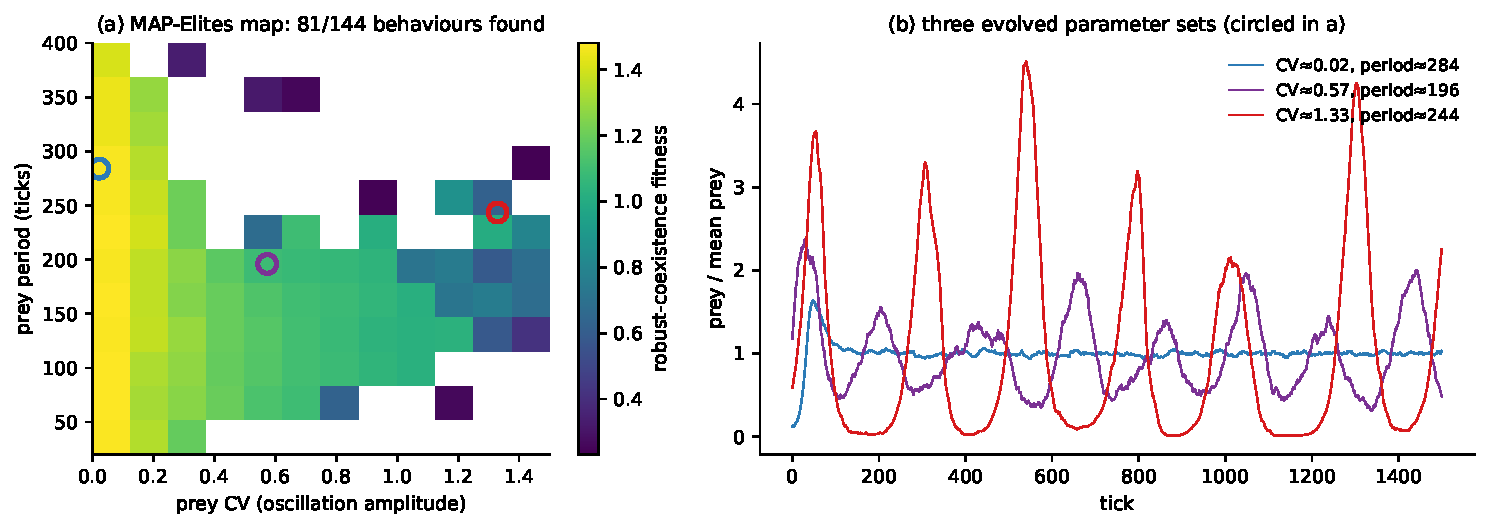
\includegraphics[width=0.9\linewidth]{qd_map.pdf}
\caption{(a) MAP-Elites archive over prey CV $\times$ period ($100^2$ cells, 1500 ticks, 3 seeds per genome);
colour is robust-coexistence fitness. (b) Prey time series (normalised) of three evolved genomes circled in (a).}
\label{fig:qd}
\end{figure*}

\subsection{Harvest control}\label{sec:control}
We now treat harvesting as the control input $u$ (Fig.~\ref{fig:loops}) acting on the stable regime
(open loop) and on the cycling regime (closed loop).

\begin{figure}[!htbp]
\centering\resizebox{\linewidth}{!}{% Shared TikZ figure: causal-loop diagram of the ecosystem (used by paper and guide)
\begin{tikzpicture}[
  node distance=2.6cm, >=Stealth,
  stock/.style={draw, rounded corners=3pt, minimum width=2.3cm, minimum height=0.9cm, font=\small\bfseries, thick},
  lbl/.style={font=\footnotesize, inner sep=1pt},
  plusarrow/.style={->, thick, draw=black!70},
  minusarrow/.style={->, thick, draw=red!70!black, dashed}]
  \node[stock, fill=green!15]  (V) {Vegetation};
  \node[stock, fill=yellow!25, right=of V] (X) {Prey};
  \node[stock, fill=red!15, right=of X] (Y) {Predators};
  \node[stock, fill=blue!10, below=1.5cm of Y, font=\small] (H) {Harvest (control input $u$)};
  % food chain
  \draw[plusarrow] (V) to[bend left=25] node[lbl, above] {$+$ food} (X);
  \draw[minusarrow] (X) to[bend left=25] node[lbl, below] {$-$ grazing} (V);
  \draw[plusarrow] (X) to[bend left=25] node[lbl, above] {$+$ food} (Y);
  \draw[minusarrow] (Y) to[bend left=25] node[lbl, below] {$-$ predation} (X);
  % self loops
  \draw[plusarrow] (X.north west) ++(0.25,0) arc[start angle=200, end angle=-20, radius=0.42] node[lbl, pos=0.5, above] {$+$ births};
  \draw[plusarrow] (V.north west) ++(0.25,0) arc[start angle=200, end angle=-20, radius=0.42] node[lbl, pos=0.5, above] {$+$ regrowth};
  \draw[minusarrow] (Y.north west) ++(0.25,0) arc[start angle=200, end angle=-20, radius=0.42] node[lbl, pos=0.5, above] {$-$ starvation};
  \draw[minusarrow] (H) -- node[lbl, right] {$-$ removal} (Y);
  \draw[minusarrow] (H.west) -| node[lbl, pos=0.75, left] {$-$} (X.south);
  \draw[->, thin, draw=blue!60, dotted, thick] (Y.south east) to[bend left=50] node[lbl, right, text=blue!60!black] {measure $y$ (feedback)} (H.east);
\end{tikzpicture}
}
\caption{Causal-loop view of the ecosystem with harvest as control input. Solid: reinforcing ($+$);
dashed: opposing ($-$); dotted: measurement used by feedback control.}
\label{fig:loops}
\end{figure}

\paragraph{Constant effort and the Volterra principle.} Removing a fixed fraction $E$ per tick behaves as
LV theory predicts (Fig.~\ref{fig:effort}). Harvesting prey does not lower the prey level: it
\emph{lowers predators} (from \HzeroPred{} to \PreyHpred{} at $E=0.01$) while prey stay at or slightly above
their unharvested level (\PreyHprey{} vs \HzeroPrey), because $x^\ast=g/(cb)$ does not contain the prey's
growth rate. Harvesting both species at $E=\VoltE$ raises prey to \VoltPrey{} and cuts predators to
\VoltPred: Volterra's explanation for the rise of predatory fish when Adriatic fishing stopped during the
First World War \cite{volterra1926}. The largest prey yield compatible with coexistence in every seed is
\MSYXyield{} prey/tick at $E=\MSYXeffort$; from $E=\EcollX$ predators are lost, after which the prey-only
system follows a Schaefer curve \cite{schaefer1954} with maximum yield \FreeXyield{} at $E=\FreeXeffort$.
The predator yield peaks at \MSYYyield{} per tick ($E=\MSYYeffort$), and predators vanish from
$E=\EcollY$.

\begin{figure*}[!tp]
\centering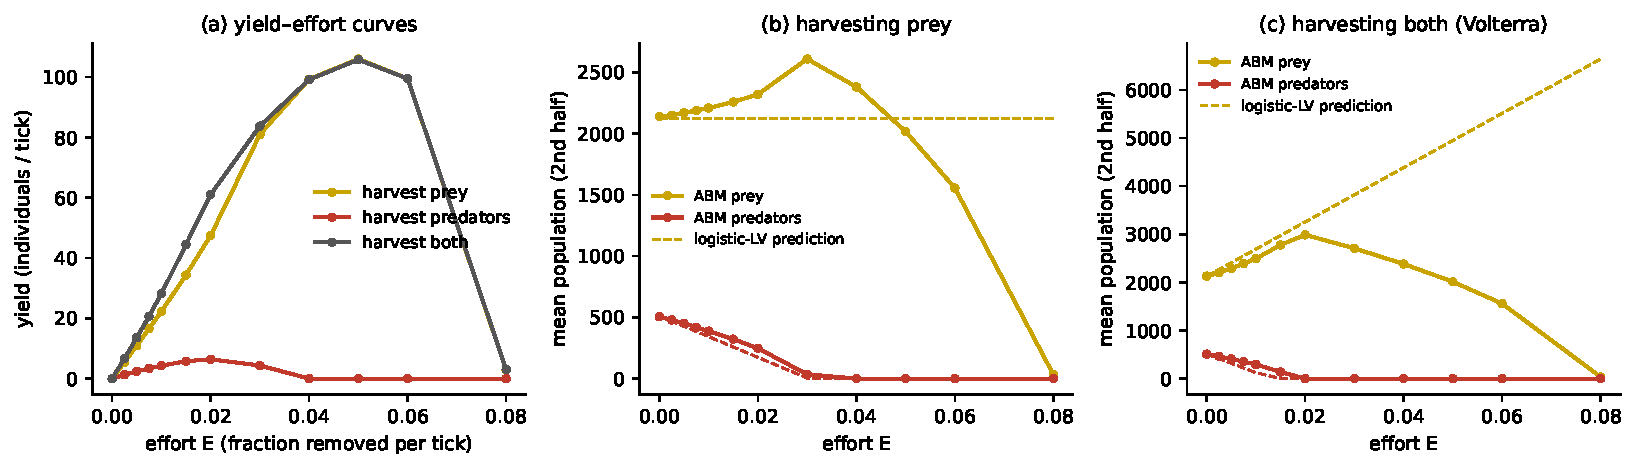
\includegraphics[width=0.95\linewidth]{harvest_effort.pdf}
\caption{Constant-effort harvesting in the stable regime (E6a; 5 seeds, 3000 ticks). (a) Yield vs effort.
(b,c) Mean populations vs effort when harvesting prey and both species; dashed: logistic-LV
equilibrium calibrated without harvest, valid only while predators persist.}
\label{fig:effort}
\end{figure*}

\paragraph{Constant quota: abrupt collapse.} A quota $Q$ ignores the state. Up to $Q=\QmaxX$ prey/tick
(switched on at $t=500$) the system absorbs it, yielding exactly $Q$ with predators reduced to
\QmaxXpred{} (Fig.~\ref{fig:quota}). One step further, at $Q=\QcollX$, only \QcollXp\% of seeds survive,
and at $Q=80$ both species are extinct in every seed. The quota sustains a higher yield than constant effort
(\QmaxX{} vs \MSYXyield) precisely because it keeps taking when the stock declines, which is also why its
failure is total rather than gradual: the harvested fraction $Q/x$ grows as $x$ falls, a destabilising
feedback \cite{clark1990}. Effort harvesting has the opposite, stabilising feedback built in; past its limit
it loses the predators but the prey persist. For predators the safe quota is \QmaxY{} per tick and
$Q=\QcollY$ is already lethal.

\begin{figure}[!htbp]
\centering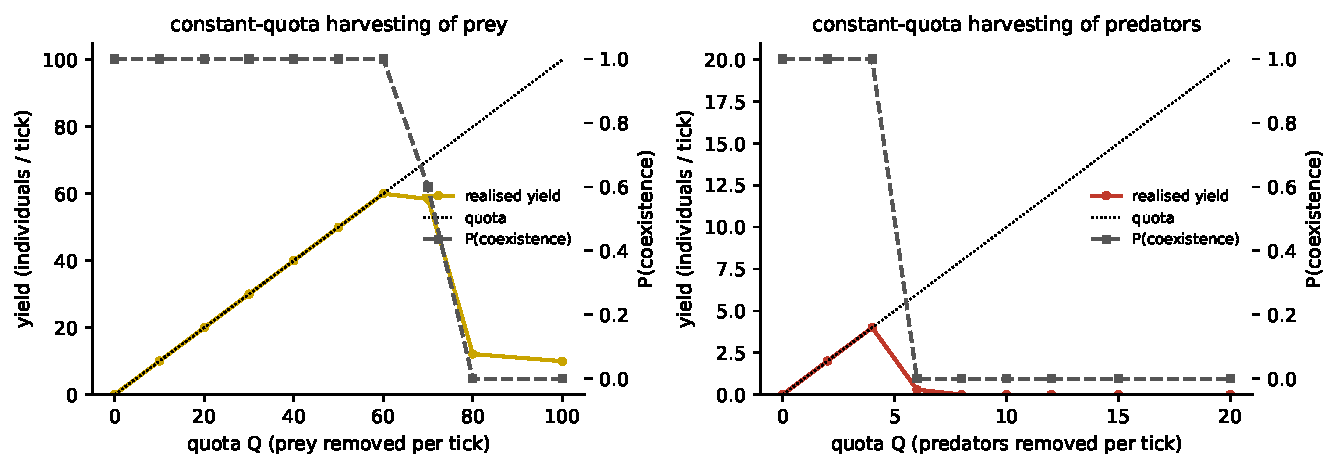
\includegraphics[width=\linewidth]{harvest_quota.pdf}
\caption{Constant-quota harvesting (E6b; 5 seeds; quota from $t=500$): realised yield and probability of
coexistence.}
\label{fig:quota}
\end{figure}

\paragraph{Proportional feedback suppresses cycles.} In the cycling regime we switch on
$u=K_p\,\max(y-r,0)$ on predators at $t=1500$ (Fig.~\ref{fig:feedback}). Even a small gain is effective:
with $r=\FBsetA$ the predator CV after switch-on falls from \FBAcvZero{} to \FBAcvTwo{} at $K_p=0.2$ and
the prey CV from \FBAcvpZero{} to \FBAcvpTwo, with coexistence in all seeds. The controller caps predator
peaks, removing the delayed overshoot that drives the cycle; prey, though not measured, are stabilised
through the coupling. Three textbook features of feedback \cite{astrom2008} appear. First, a
\emph{steady-state error}: the predator mean is \FBAmeanSmall{} at $K_p=0.02$, \FBAmeanTwo{} at $K_p=0.2$
and \FBAmeanOne{} at $K_p=1$ against a target of \FBsetA. Second, \emph{actuator saturation}: harvesting
can only remove animals, so below the target the loop is open. Third, a gain--effort trade-off: the
harvest the controller must take grows with gain and saturates around \FBAyieldTwo{} predators/tick.

Controlling the prey instead reveals a hidden-state hazard: holding prey at $r=800$ with $K_p\ge0.5$
drives predators extinct in every seed, because the target lies below the prey density predators need to
break even. A set point on one state variable can destroy an unmeasured one---the ecological analogue of
unstable internal dynamics behind a well-regulated output.

\begin{figure*}[!tp]
\centering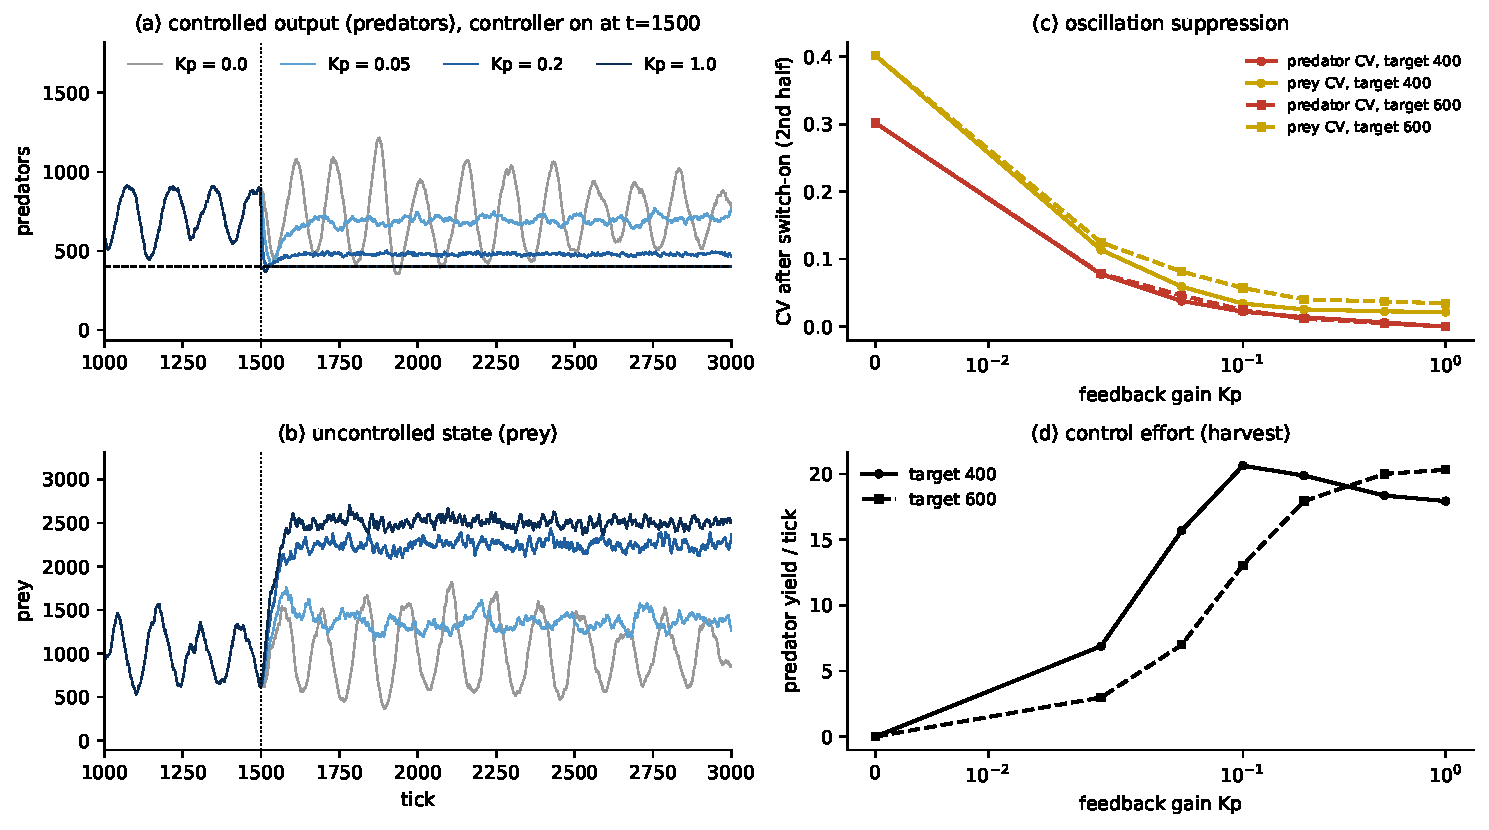
\includegraphics[width=0.95\linewidth]{feedback.pdf}
\caption{Proportional feedback on predators in the cycling regime (on at $t=1500$; E6c, 5 seeds,
4000 ticks): controlled output, prey, post-switch CV vs gain, and harvest taken.}
\label{fig:feedback}
\end{figure*}

\paragraph{Open versus closed loop at equal yield.} Comparing constant predator effort with feedback
($K_p=0.2$, varying $r$; E6d, both from $t=0$) at matched predator yields of \ODyLo--\ODyHi{} per tick, the
feedback policy leaves a prey CV that is on average \ODratio{} times that of the open-loop policy
(Fig.~\ref{fig:openclosed}). Constant effort also damps cycles, since it adds predator mortality, but never
brings the prey CV below \ODeffCVmin{} in the tested range, whereas feedback reaches \ODfbCVmin.

\begin{figure}[!htbp]
\centering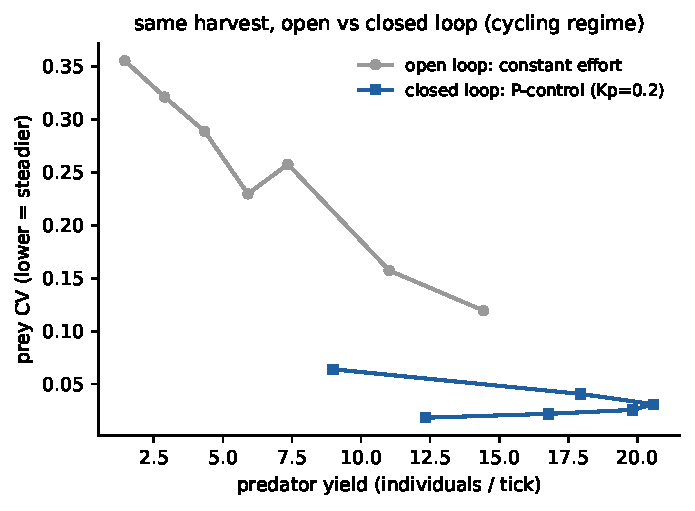
\includegraphics[width=0.85\linewidth]{open_vs_closed.pdf}
\caption{Prey variability vs predator yield for open-loop constant effort and closed-loop proportional
control, cycling regime (E6d; 5 seeds).}
\label{fig:openclosed}
\end{figure}

\subsection{Stability probe}
Removing half of the predators at $t=1500$ (Fig.~\ref{fig:shocks}) produces, in the stable regime, a prey
outbreak peaking $\approx\ShockSpreyPeak$ above control after \ShockSpreyPeakT{} ticks, and the deviation
envelope decays by a factor $e$ in $\approx\ShockStau$ ticks (\ShockSn{} seeds). The fitted chain model
predicts a damping time of \ShockModelTau{} ticks: the impulse response measured on agents and the
eigenvalue computed from the reduced model agree. In the cycling regime the same shock does not simply
decay: it resets the phase of the cycle in all seeds at once, and the mean deviation keeps oscillating for
the full 900 observed ticks (Fig.~\ref{fig:shocks}b), the signature of a very weakly damped oscillatory
mode---consistent with the noise-sustained cycles of Sec.~\ref{sec:quasi}.

\begin{figure*}[!tp]
\centering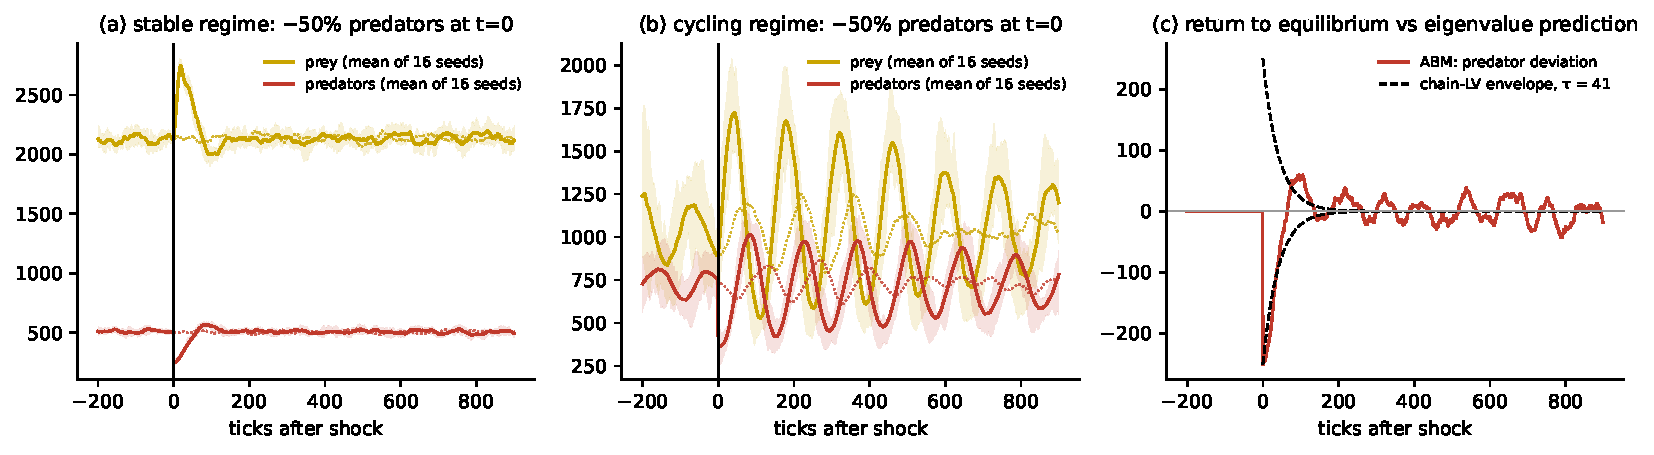
\includegraphics[width=0.95\linewidth]{shocks.pdf}
\caption{Mean response (16 seeds) to removing 50\% of predators or doubling prey at $t=1500$, relative to
unshocked runs with the same seeds.}
\label{fig:shocks}
\end{figure*}

\subsection{Optimising the harvest policy}\label{sec:yield}
Finally we let a genetic algorithm design the prey-harvest policy: the genome holds the controller type
(effort, quota or feedback) and its parameters, and fitness is the mean prey yield per 1000 cells in the
second half of a 1500-tick run on a $100^2$ grid (3 training seeds, population 32, \Ygens{} generations,
\Yevals{} simulations). No stability or coexistence term was included. The search converged on
\YmodeName{} with $E=\Yeffort$, a training fitness of \Ytrain{} prey per tick per 1000 cells. Among
policies that kept both species alive on all training seeds, the best effort, quota and feedback designs
reached \YbestEff, \YbestQuo{} and \YbestFb{}, respectively. Feedback was abandoned early: only 11 of
632 genomes used it, and 9 of those had set points above the prey level of a $100^2$ world, so the
controller was idle. The GA's verdict on feedback is therefore uninformative, not negative.

Re-validated on 10 fresh seeds, the same genome scored only \Yval{}: predators survived in \Ycoex\% of
seeds (mean \YmeanPred{} predators). The evolved effort sits just below the point where predators are lost
in E6a, the edge of the coexistence region, where the outcome depends on chance. This is the expected
behaviour of an optimiser given a yield-only objective with few seeds: it climbs to the boundary of the
feasible region and \emph{overfits} the training noise. Robust management requires putting the constraint
(coexistence, variability) into the objective and evaluating it over many stochastic realisations---the
same lesson as the specification gaming of Sec.~\ref{sec:opt}, now with an economic objective.



